\documentclass{report}

\usepackage[utf8]{inputenc}
\usepackage[francais]{babel}
\usepackage[T1]{fontenc}
\usepackage{graphicx}
\usepackage{xcolor}
\usepackage{amsmath}
\usepackage{amssymb}

\title{Rapport du projet de graphes}
\author{Baptiste Prunot
\and Amaury Sauvage
\and Raphael Pinto
\and Hugo Ouertani
\and Cyril Vandenbosshe}
\date{\today}

\begin{document}
	\maketitle

	\part*{Introduction} 
	
	\part{Generation des graphes et mode manuel}
		\section{generation des graphes}
			\paragraph{\textcolor{blue}{graphe de la carte}}
			Le graphe de la carte est la base sur laquelle vont \^etre g\'en\'er\'es le graphe des zombies, et celui des licornes.
			
			le graphe a la particularit\'e de repr\'esenter une carte avec des cases hexagonales. De ce fait, sa g\'en\'eration a entrain\'e quelques particularit\'es.
			
			Pour expliquer la methode utilis\'ee pour g\'en\'erer le graphe nous nous appuierons sur l'exemple d'une carte de taille 2.
			
			\begin{center}
				\framebox[7cm]{
					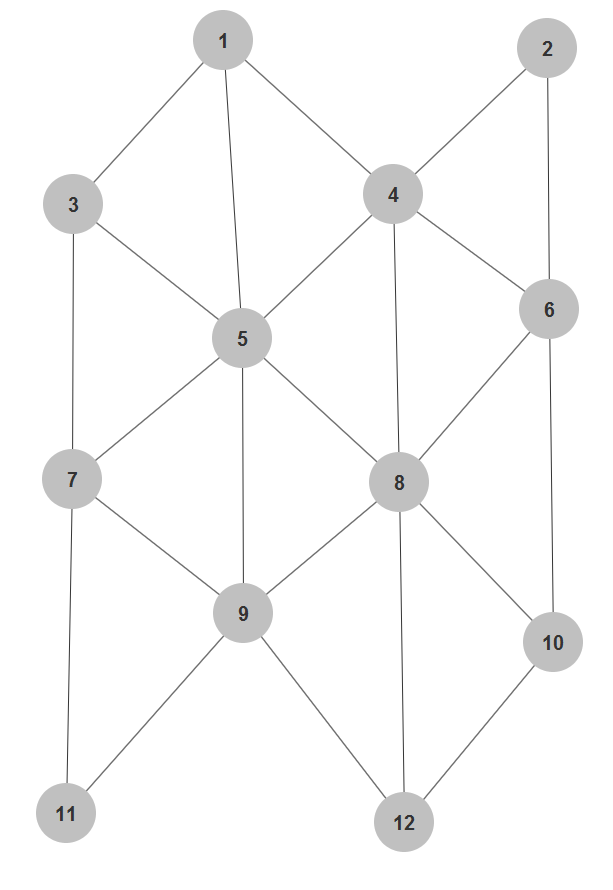
\includegraphics[scale=0.30]{Images/Graphe.png}
				}
			\end{center}
			
			Si nous choisissons le sommet 1, nous remarquons qu'il est li\'e \'a aux sommets suivants :
			
			\itemize{
				\item[*] le sommet 3 ce qui correspond \'a sommet+2 soit :
				
				
				\fbox{
				$sommet+tailleGraphe$
				}
				\item[*] le sommet 5 ce qui correspond \'a sommet+4 soit :
				
				
				\fbox{
				$sommet+tailleGraphe\times2$
				}
				\item[*] le sommet 4 ce qui correspond \'a sommet+3 soit : 
				
				
				\fbox{
				$sommet+tailleGraphe+1$
				}
			}
			
			On pourrait donc conclure que pour generer le graphe il suffirait de lier chaque sommet avec les observations faites ci-dessus. Cependant, bien que lier un sommet
			
			
			
			
			
			
			\paragraph{graphe des licornes}
			\paragraph{graphe des zombies}
	\part{mode automatique}
	
\end{document}